\section{Results} \label{results}

This section highlights sample navigation results from a high fidelity closed loop simulation. Table~\ref{tab:sim_setup} lists the relevant navigation sensor parameters used for simulation. The simulation includes full image rendering using the Rendering and Camera Emulator (RCE)~\cite{rce} and surrogate Titan terrain using a DEM of the Namib desert.\cite{schilling2019} All simulations include ETS/image processing and closed loop guidance and control.  

\begin{table}[htbp]
	\fontsize{10}{10}\selectfont
    \caption{Simulation setup for navigation performance analysis}
   \label{tab:sim_setup}
        \centering 
   \begin{tabular}{| c | c |} % Column formatting, 
      \hline 
      Sensor Parameter & Specification (1$\sigma$)  \\
      \hline 
        Accel bias & 40 $\mu$g \\
        Accel scale factor & 120 PPM \\
        Accel velocity random walk & 0.2 mm/s/$\sqrt{hr}$ \\
        Accel acceleration random walk & 0.05 $\mu$g/$\sqrt{hr}$ \\
        Accel white noise & 0.198 mm/s  \\
        Accel misalignment & 0.03$^\circ$ per axis \\
        Gyro bias & 0.005$^\circ$/hr  \\
        Gyro scale factor & 40 PPM  \\
        Gyro angle random walk & 0.005 $^\circ$/$\sqrt{hr}$  \\
        Gyro rate random walk & 0.017$^\circ$/hr  \\
        Gyro white noise & 0.75 $\mu$rad  \\
        Gyro misalignment & 0.03$^\circ$  \\
        Lidar white noise & 2 cm  \\
        Lidar pointing & 0.05$^\circ$  \\
        Pressure white noise & 2.7 mbar  \\
        Pressure CFD model error & 6.67\%  \\
      \hline
   \end{tabular}
\end{table}

\subsection{Gyrocompassing}

A Monte Carlo simulation was run to characterize the gyrocompassing performance using the model described in the Design section. The initial heading error was drawn from a normal distribution with zero mean and standard deviation of 2$^\circ$, a conservative worst-case initial heading error following \ac{EDL}. 500 cases were run using parameters outlined in Table~\ref{tab:sim_setup} and the navigation filter was configured to process data from both \acp{IMU}. Figure~\ref{fig:gyrocompassing} illustrates heading error as a function of time for all cases, showing consistent errors between the empirical Monte Carlo error (green) and filter uncertainty (red). The baseline CONOP is to gyrocompass for 60 minutes, allowing the filter to squeeze heading error to less than 1$^\circ$ (3$\sigma$). 

\begin{figure}[htbp]
	\centering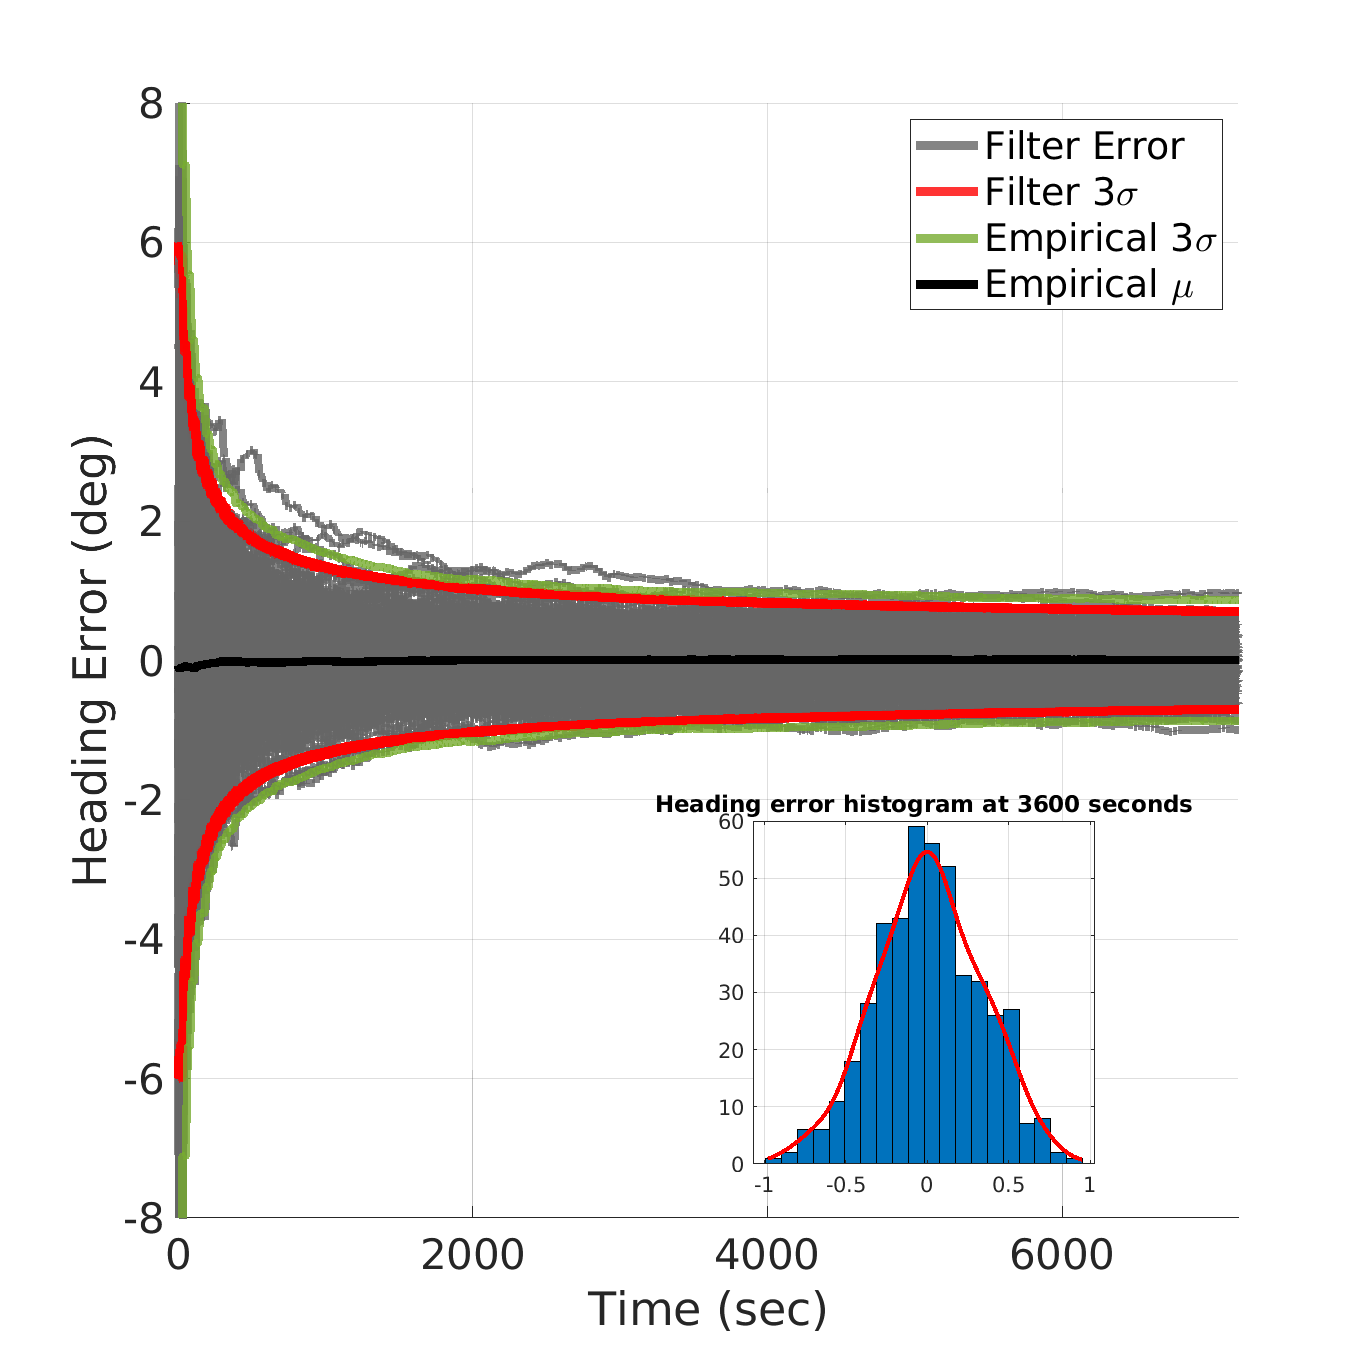
\includegraphics[width=4.5in]{content/figures/gc/dual/HeadingErrorTOF.png}
	\caption{Heading initialization using 2 IMUs}
	\label{fig:gyrocompassing}
\end{figure}

\subsection{Leapfrog}

A Monte Carlo of the Scout and Leapfrog were run to characterize the performance of long distance traverse navigation. The initial heading error was drawn from a normal distribution with zero mean and standard deviation of 0.4$^\circ$ for both the Scout and Leapfrog flights, representing conservative initial heading errors after gyrocompassing completes, leading to initial relative heading errors between the two flights of $\sim$1.7$^\circ$ (3$\sigma$). The root sum square (RSS) of the lateral position errors for 10 of the Leapfrog cases are illustrated in Figure~\ref{fig:leapfrog}. The colors represent lateral errors in different frames including NED (black), TOF (blue), and the breadcrumb relative error (red). When traversing down range the position errors are composed of error due to absolute heading error, which scales linearly with lateral distance, and random walk error from \ac{VIO}. Lateral errors in the NED frame represent absolute (i.e. total) position error, while errors in the TOF represent only the random walk component (by definition, the TOF does not contain position error due to global heading errors). Finally, and most important for Dragonfly, are the breadcrumb relative errors depicted in red. These errors are also in the NED frame but are relative to the historic breadcrumb in the nav filter. The breadcrumb relative errors are dominated by relative heading error between flights and a random walk between breadcrumbs. The breadcrumb relative errors remain small as the vehicle retraces the climb and cruise segments of the Scout flight but begin growing after losing historic breadcrumbs when the vehicle flies over the landing site. After scouting a new candidate landing zone the vehicle turns around and flies back towards the landing site causing the breadcrumb relative errors to decrease. Finally, when the vehicle descends and reaches the terminal breadcrumb the breadcrumb relative errors are small enough to ensure the reference image selected by ETS will contain sufficient image overlap to produce a valid correlation and displacement measurement. The breadcrumb relative errors are reduced to < 5 m after processing one or more historic breadcrumb measurements to enable precision landings.

\begin{figure}[htbp]
	\centering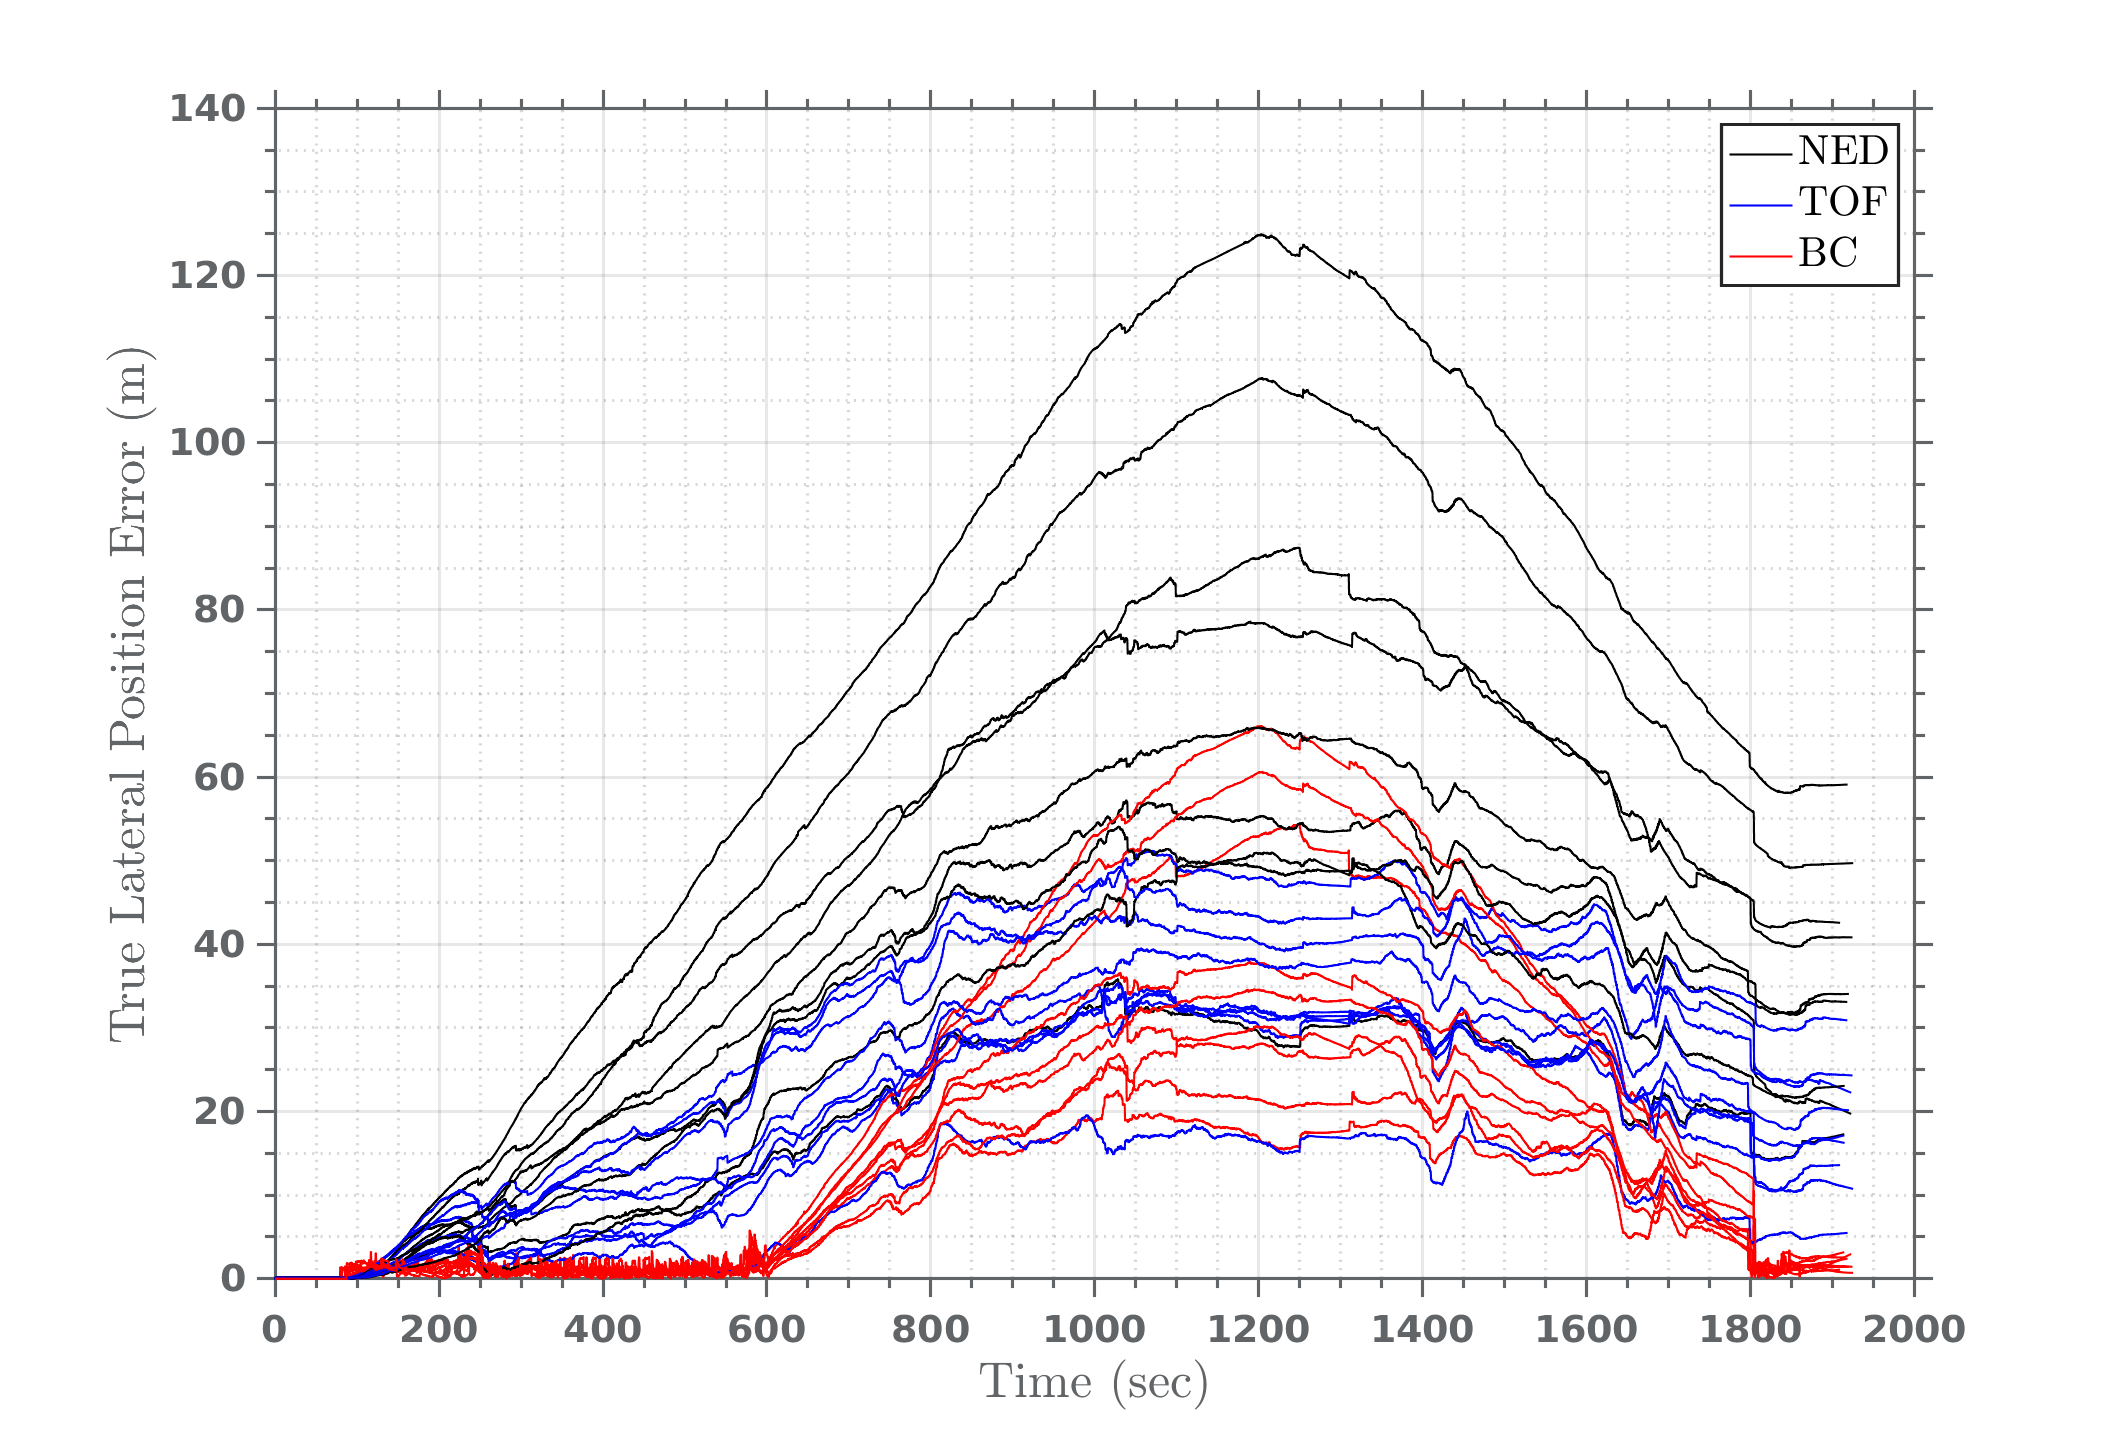
\includegraphics[width=5in]{content/figures/pos_err_all_frames.png}
	\caption{Lateral position errors in NED (black), TOF (blue), and relative to the historic BC in the nav filter (red).}
	\label{fig:leapfrog}
\end{figure}